\documentclass[12pt]{article}
%Imports
\usepackage{graphicx,abstract,epstopdf,times,authblk,geometry,fancyhdr,etoolbox,caption,sectsty,float, amsmath}
\usepackage[sort,round]{natbib}

%Margins
\newgeometry{top=2cm,left=2.5cm,right=2.5cm,bottom=4.5cm}

%Header
\addtolength{\headheight}{1.5cm}
\pagestyle{fancyplain}
\lhead{
\includegraphics[height=1.3cm]{src/logo.eps} Chair of Computation in Engineering}
\rhead{Software-Lab 2015}
\renewcommand{\headrulewidth}{0pt}

%Layout
\renewcommand\Authfont{\fontsize{10pt}{9pt}\selectfont }
\renewcommand\Affilfont{\fontsize{10pt}{9pt}\selectfont }
\renewcommand\Authands{, }
\renewcommand{\abstractname}{\vspace{-\baselineskip}}
\renewcommand{\abstracttextfont}{\fontsize{10pt}{12pt}\selectfont\noindent\textbf{Abstract. }}
\date{\vspace{-\baselineskip}\vspace{-\baselineskip}}
\captionsetup{font=small}
\allsectionsfont{\fontsize{12pt}{14pt}\selectfont\bfseries }
\renewcommand{\arraystretch}{1.8}
\AtBeginEnvironment{tabular}{\fontsize{10pt}{9pt}\selectfont}
\bibliographystyle{src/agsm}
\newcommand\emails{\affil[ ]}

\usepackage[colorinlistoftodos]{todonotes}

% For our todos we use the following colorcode:
% intern: only internal info, dont care
% urgent: all please have a look at it
% done: task solved, but would not mind a second person having a look at it

% the following todo commands take the arguments 
% \todo...[options]{author}{todomessage}
% options are the common options from the todonotes package and are an optional parameter
% for \todoin...[options]{author}{todomessage}{section}
% where todoin marks a whole section for refactoring or similar. 
\newcommand{\tododone}[3][noinline]{\todo[#1, author = #2, color=green!40]{\textit{#3}}}
\newcommand{\todointern}[3][noinline]{\todo[#1, author = #2, color=blue!40]{#3}}
\newcommand{\todourgent}[3][noinline]{\todo[#1, author = #2, color=red!40]{\textbf{#3}}}
\newcommand\todoindone[4][]{\todo[inline, author = #2, caption={#3}, #1, color=green!40]{
\begin{minipage}{\textwidth-4pt}\underline{#3}\\ \textit{#4}\end{minipage}}}
\newcommand\todoinintern[4][]{\todo[inline, author = #2, caption={#3}, #1, color=blue!40]{
\begin{minipage}{\textwidth-4pt}\underline{#3}\\  #4\end{minipage}}}
\newcommand\todoinurgent[4][]{\todo[inline, author = #2, caption={#3}, #1, color=red!40]{
\begin{minipage}{\textwidth-4pt}\underline{#3}\\ \textbf{#4}\end{minipage}}}


\begin{document}

%------------------------------------------------------------------------------------------------------------------------
% Title and Abstract
%------------------------------------------------------------------------------------------------------------------------
\title{Integrated Parametric Shaft Generator}

%Add/Remove authors as you please
%Numbers in [] correspond to affiliations below
%\emails must be before \affils

\author[1]{Mohamed Khalil}
\author[1]{Zeno Korondi}
\emails{mohamed.khalil@tum.de, korondi.zeno@gmail.com}
\author[2]{Mohamed Elhaddad}
\author[2]{Tino Bog}
\emails{mohamed.elhaddad@tum.de, tino.bog@tum.de}

\affil[1]{Master's Computational Mechanics students, Technical University in Munich}
\affil[2]{Chair of Computation in Engineering, Technical University in Munich}

\maketitle

\begin{abstract}
The Integrated Parametric Shaft Generator (IPSG) is an integrated framework for designing and analysis of shafts, a vital component in a plethora of mechanical applications. This framework allows the user to flexibly build the shaft's geometry and mount common shaft features such as fillets, chamfers and keyways, as well as apply the necessary loads at given sections and conduct a structural finite elements analysis, all under one graphical user interface (GUI). The analysis is being conducting using the finite cell method (FCM) for higher order FE analysis, developed at the Chair of Computation in Engineering at Technical University in Munich. This work has also involved implementing a polar cell grid to conform to the cylindrical base geometry of the shafts, aiming to reduce the complexity of the FCM analysis using cartesian grid. The efficiency of both methods have been compared and presented in this work.
\end{abstract}



%------------------------------------------------------------------------------------------------------------------------
% Introduction
%------------------------------------------------------------------------------------------------------------------------
\section{Introduction}
In the introduction we should talk about:
\begin{itemize}
\item Shafts
\item Shaft analysis methods (analytical, FEM, etc.)
\end{itemize}

% This file can be used as a template. In such a case, notice that at the left-hand side MS-Word provide a Navigation tool, which will allow you to know whether you are setting the right headings.\\
% 
% Please send a final \LaTeX and PDF file of your paper to your supervisors before the final presentation. The maximum length of the paper should not exceed 10 pages, including tables, figures and references. 



%------------------------------------------------------------------------------------------------------------------------
% Motivation
%------------------------------------------------------------------------------------------------------------------------
\section{Motivation}
In the motivation, we should write a line or two about why we want to do this. Examples:
\begin{itemize}
\item An integrated environment of analysis and design compared to separate CAD and FEM packages
\item Using HOFEM to obtain a conforming elements to the shaft's geometry and possibly for the features as well since they all have a closed-form geometric description
\end{itemize}

% Students should also prepare a Poster as part of the final documentation. Please, remember that the poster is the first contact for the other students with your topic, should wake up their attention and guide them to the paper to get more information. Poster and paper are NOT the same document, but two different ways to present your results.


%------------------------------------------------------------------------------------------------------------------------
% Scope
%------------------------------------------------------------------------------------------------------------------------
\section{Scope}
\subsection{The Finite Cell Method}
\label{fcm_subsection}
Finite cell method is an embedded domain method in which the subject domain under investigation is \emph{embedded} in a grid of cartesian finite cells as shown in figure~\ref{fig:fcmConcept}. Cells that cross the boundary of the domain are partitioned by a bisecting their sides (forming bi-tree in 1D, quad-tree in 2D and octree in 3D) for a given number of times, known as the partioning depth. For every cell, the equation system is evaluated at a number of integration points $n$ using equation \ref{eq:fcm_equation}

\begin{equation}
\label{eq:fcm_equation}
\delta W = \int_{\Omega} \delta v \textbf{B}^T \textbf{C} \textbf{B} d\textbf{v}
	 - \int_{\Omega} \delta v \textbf{P} \alpha d\textbf{v}
	 - \int_{\Gamma} \delta v \textbf{t} \alpha d\textbf{a}
\end{equation}
where $\Omega$ is the volume of the cells' domain, $\Gamma$ is the boundary of the cells' domain, $\delta v$ and $\delta W$ are the virtual displacement and work, respectively, $\textbf{B}$ is the B matrix, $\textbf{C}$ is the constitutive law matrix, $P$ and $t$ are the body and surface loads, respectively. The distinction in the evaluation of the physical domain $\Omega_{phys}$ and the fictious domain $\Omega_{fict} = \Omega - \Omega_{phys}$ is determined by the value of $\alpha$ given by:

\begin{equation}
\label{eq:alpha_equation}
\alpha = 
\begin{cases}
    1.0 \qquad \forall x \in \Omega_{phys} \\
    \approx 0 \qquad \forall x \in \Omega_{fict}
\end{cases}
\end{equation}

\begin{figure}
  \begin{center}
    \includegraphics[width=\textwidth]{./images/fcm_concept.png}
    \caption{Schematic representing the principle of the finite cell method}
    \label{fig:fcmConcept}
  \end{center}
\end{figure}
\subsection{Higher Order Finite Elements Method}
The choice of FCM is usually associated with using HOFEM due to its robustness in representing state-variables' field with higher order functions and the ability to achieve logarithmic rates of convergence (at worst linear for non-smooth problems) by increasing the polynomial degree of the shape functions (p-refinement) compared to decreasing the edge size (h-refinement) of linear elements. In addition, the usage of the hierarchical approach of order elevation offers the versatility of formulating elements with exact conformity to the meshed topology (or highly conforming for non-definite topologies). The latter feature allows the shaft's base geometry, which is of cylinderical natrue, to be represented exactly by \emph{blending} two edges of a hexagonal element\footnote{Different features of the shaft such as fillets, keyways, etc. could also be represented by blended hexes due to their closed-form geometry description but this wasn't implemented within the scope of this work}.
Hierarchical order elevation is based on overlaying the linear shape functions $N_1$ and $N_2$ in equation \ref{eq:hierarchical}, referred to as \textit{node modes} by a hierarchy of higher order Legendre polynomials $\phi_i$ across the edges in one dimensions, referred to as \textit{edge modes}. To extend this concept in 2D and 3D, the edge modes are blended across the element by performing a tensor product with orthogonal nodal modes or edge modes, forming internal modes and face modes, respectively. Details on this topic are more thoroughly presented in \citep{hofem_script}

\begin{subequations}
\label{eq:hierarchical}
\begin{align}
N_0 &= \frac{1}{2}(1 - \xi) \\
N_1 &= \frac{1}{2}(1 + \xi) \\
N_i &= \phi_{i}(\xi, \eta)
\end{align}
\end{subequations}

In the case of a shaft, each section was represented by $n$ blended hexes extruded over its lenth. Figure \ref{fig:blended_hex} shows a quad with two edge modes, representing equations of an arc, being applied to its edges $E_0$ and $E_2$. The formulation of this blending is given in equations \ref{eq:blended_hex}.

\begin{figure}
  \begin{center}
    \includegraphics[width=200pt]{./images/blended_hex.png}
    \caption{Blended quad element}
    \label{fig:blended_hex}
  \end{center}
\end{figure}

\begin{subequations}
\label{eq:blended_hex}
\begin{align}
  x &= \sum_{i = 0}^3 N_i(\xi, \eta) X_i \nonumber \\
    &\qquad {} + \big( E_{x0}(\xi) - ( \frac{1-\xi}{2}X_0 + \frac{1+\xi}{2}X_1 ) ) \frac{1-\eta}{2} \nonumber \\
    &\qquad {} + \big( E_{x2}(\xi) - ( \frac{1-\xi}{2}X_3 + \frac{1+\xi}{2}X_2 ) ) \frac{1+\eta}{2} \\
  y &= \sum_{i = 0}^3 N_i(\xi, \eta) Y_i \nonumber \\
    &\qquad {} + \big( E_{y0}(\xi) - ( \frac{1-\xi}{2}Y_0 + \frac{1+\xi}{2}Y_1 ) ) \frac{1-\eta}{2} \nonumber \\
    &\qquad {} + \big( E_{y2}(\xi) - ( \frac{1-\xi}{2}Y_3 + \frac{1+\xi}{2}Y_2 ) ) \frac{1+\eta}{2}
\end{align}
\end{subequations}
where $X_i$ and $Y_i$ are the nodal coordinates, $N_i$ are the linear nodal modes of a quad, and $E_{xi}$ and $E_{yi}$ are the edge modes of the ith edge in x and y described by an arc with radius $R_i$, center coordinates ($X_c$, $Y_c$), start angles $\phi$ and end angle $\theta$ as shown in the following equations:

\begin{subequations}
\label{eq:edge_modes_hex}
\begin{align}
      E_{xi}(\xi) &= X_c + R_i cos( \frac{1-\xi}{2}\phi + \frac{1+\xi}{2}\theta ) \\
      E_{yi}(\xi) &= Y_c + R_i cos( \frac{1-\xi}{2}\phi + \frac{1+\xi}{2}\theta )
\end{align}
\end{subequations}

The HOFEM concept was in principle used to reduce the intensity of partitioning needed by FCM. As explained in \ref{fcm_subsection}, the cut cells need to be partitioned up to a given depth at the integration level in order to reduce the intergration error. however, using blended hexes, as formulated above, for the FCM grid cells forming a polar grid rather than a cartesian grid results in cells conforming to the base domain of the shaft and isolating the need for partitioning to the zones where the features are located, as shown in figure ~\ref{fig:fcm_grids_comparison}. The reduction in partitioning depth and locations is reflected in turn in a reduction in the number of integration points to be evaluated (which are typically high for HOFEM, usually one point more than the polynomial order)

\begin{figure}
  \begin{center}
    \includegraphics[width=\textwidth]{./images/fcm_grids_comparison.png}
    \caption{Comparison between the integration grid for cartesian FCM grid (right) and polar FCM grid (left)}
    \label{fig:fcm_grids_comparison}
  \end{center}
\end{figure}


\subsection{Data Structure}
% How the program was structured, how the data was stored, transmitted between the python interface and Adhoc++, boost wrapping of the analysis kernel. A UML diagram would be good here.

The IPSG is composed of three major blocks:
\begin{itemize}
\item{Shaft Data}: This block is scripted in Python language and is concerned with the data storage of the shaft details as well as its components (loads, features, etc.)
\item{Analysis Kernel}: This block is scripted in C++ as part of Adhoc++ and is concerned with conducting FCM analysis on the shaft, obtaining its geometry from STL files generated by OpenCascade libraries utilized by the GUI.
\item{GUI}:
\tododone[inline]{Mohamed}{responsible for \textit{GUI}: Zeno}
\end{itemize}

The link between the first two blocks is indicated in the UML class diagram in figure ~\ref{uml}. The interface \emph{AnalysisKernelFcmWrapper} was responsible for wrapping the functionalities of the c++ class \emph{AnalysisKernelFcm} to make them accessible through the corresponding Python class \emph{ShaftAnalysisKernel} using \emph{boost::python} library.

\begin{figure}
  \begin{center}
    \includegraphics[width=\textwidth]{./images/uml.png}
    \caption{UML Diagram for Data Structure of the Shaft and Analysis Kernel}
    \label{fig:uml}
  \end{center}
\end{figure}
\section{Tools Used}
Different tools we have used for the software lab. Last slide of the first presentation. python and c++ for programming, VTK and OC for GUI and results visualisation, boost libraries for wrapping, etc.


%------------------------------------------------------------------------------------------------------------------------
% Results
%------------------------------------------------------------------------------------------------------------------------
\section{Results}
When we get results, I will write something here


%------------------------------------------------------------------------------------------------------------------------
% Conclusion
%------------------------------------------------------------------------------------------------------------------------
\section{Conclusion}
summary of the work and comments on the results. Future work of this project etc.


%------------------------------------------------------------------------------------------------------------------------
% Conclusion
%------------------------------------------------------------------------------------------------------------------------
\include{./sections/Inf_Appendix}


%------------------------------------------------------------------------------------------------------------------------
% Citation
%------------------------------------------------------------------------------------------------------------------------
\bibliography{softwarelab}

\end{document}


%------------------------------------------------------------------------------------------------------------------------
% TINO's REMARKS - SHALL BE OMITTED AFTER FINISHING THE REPORT
%------------------------------------------------------------------------------------------------------------------------

%\section{Scope (Paper preparation)}
%
%Please ensure that the margins of the page are set for: 3 cm at the top and 2.5cm at the bottom, right and left margins. The text should be justified to occupy the full line width, so that the right margin is not ragged, with words hyphenated as appropriate. As of 2007 MS-Word supports Auto-Hyphenation.
%Use 10-point type for the name(s) of the author(s) and 10-point type for the address(es) and the abstract. For the main text, please use 12-point type and single-line spacing. The font style must be Times. Italic type may be used to emphasize words in running text. Bold type and underlining should be avoided. 
%
%\subsection{Headings}
%
%Headings should be capitalized (i.e., nouns, verbs, and all other words except articles, prepositions, and conjunctions should be set with an initial capital) and should, with the exception of the title, be aligned to the left. Words joined by a hyphen are subject to a special rule. If the first word can stand alone, the second word should be capitalized. The font sizes are given in Table \ref{table:example}.
%
%\begin{table}
%\begin{center}
%\caption{Font sizes in Tables should be 10 point with the bold headings.}
%\label{table:example}
%\begin{tabular}{|c|c|c|} \hline
%\textbf{Heading level} & \textbf{Example} & \textbf{Font size and style} \\ \hline 
%Title (centered) & Lecture Notes... & 14 point, bold \\ \hline
%1st-level heading & 1 Introduction & 12 point, bold \\ \hline
%2nd-level heading & 2.1 Printing Area & 12 point, bold \\ \hline
%3rd-level heading & Headings.  Text follows... & 12 point, bold \\ \hline
%4th-level heading & Remark.  Text follows... & 10 point, italic \\ \hline
%\end{tabular}
%\end{center}
%\end{table}
%
%\subsection{Figures}
%Figures should be numbered and should have a caption which should always be positioned under the figures, in contrast to the caption belonging to a table, which should always appear above the table. Please centre the captions between the margins and set them in 11-point type. 
%
%\begin{figure}[!ht]
%	\begin{center}
%	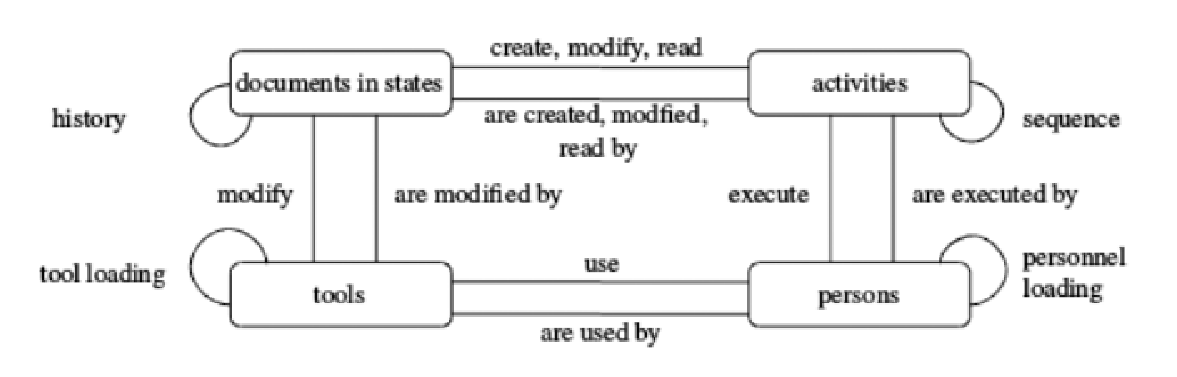
\includegraphics[width=140mm]{figure1.eps}
%	\caption{Sets and Relations of a Planning Process Model}
%	\label{figure:example1}
%	\end{center}
%\end{figure}
%
%Colour pictures should be displayed in grey-scale, unless they would be the result of simulations where colours have an extra meaning.
%
%\begin{figure}[!ht]
%	\begin{center}
%	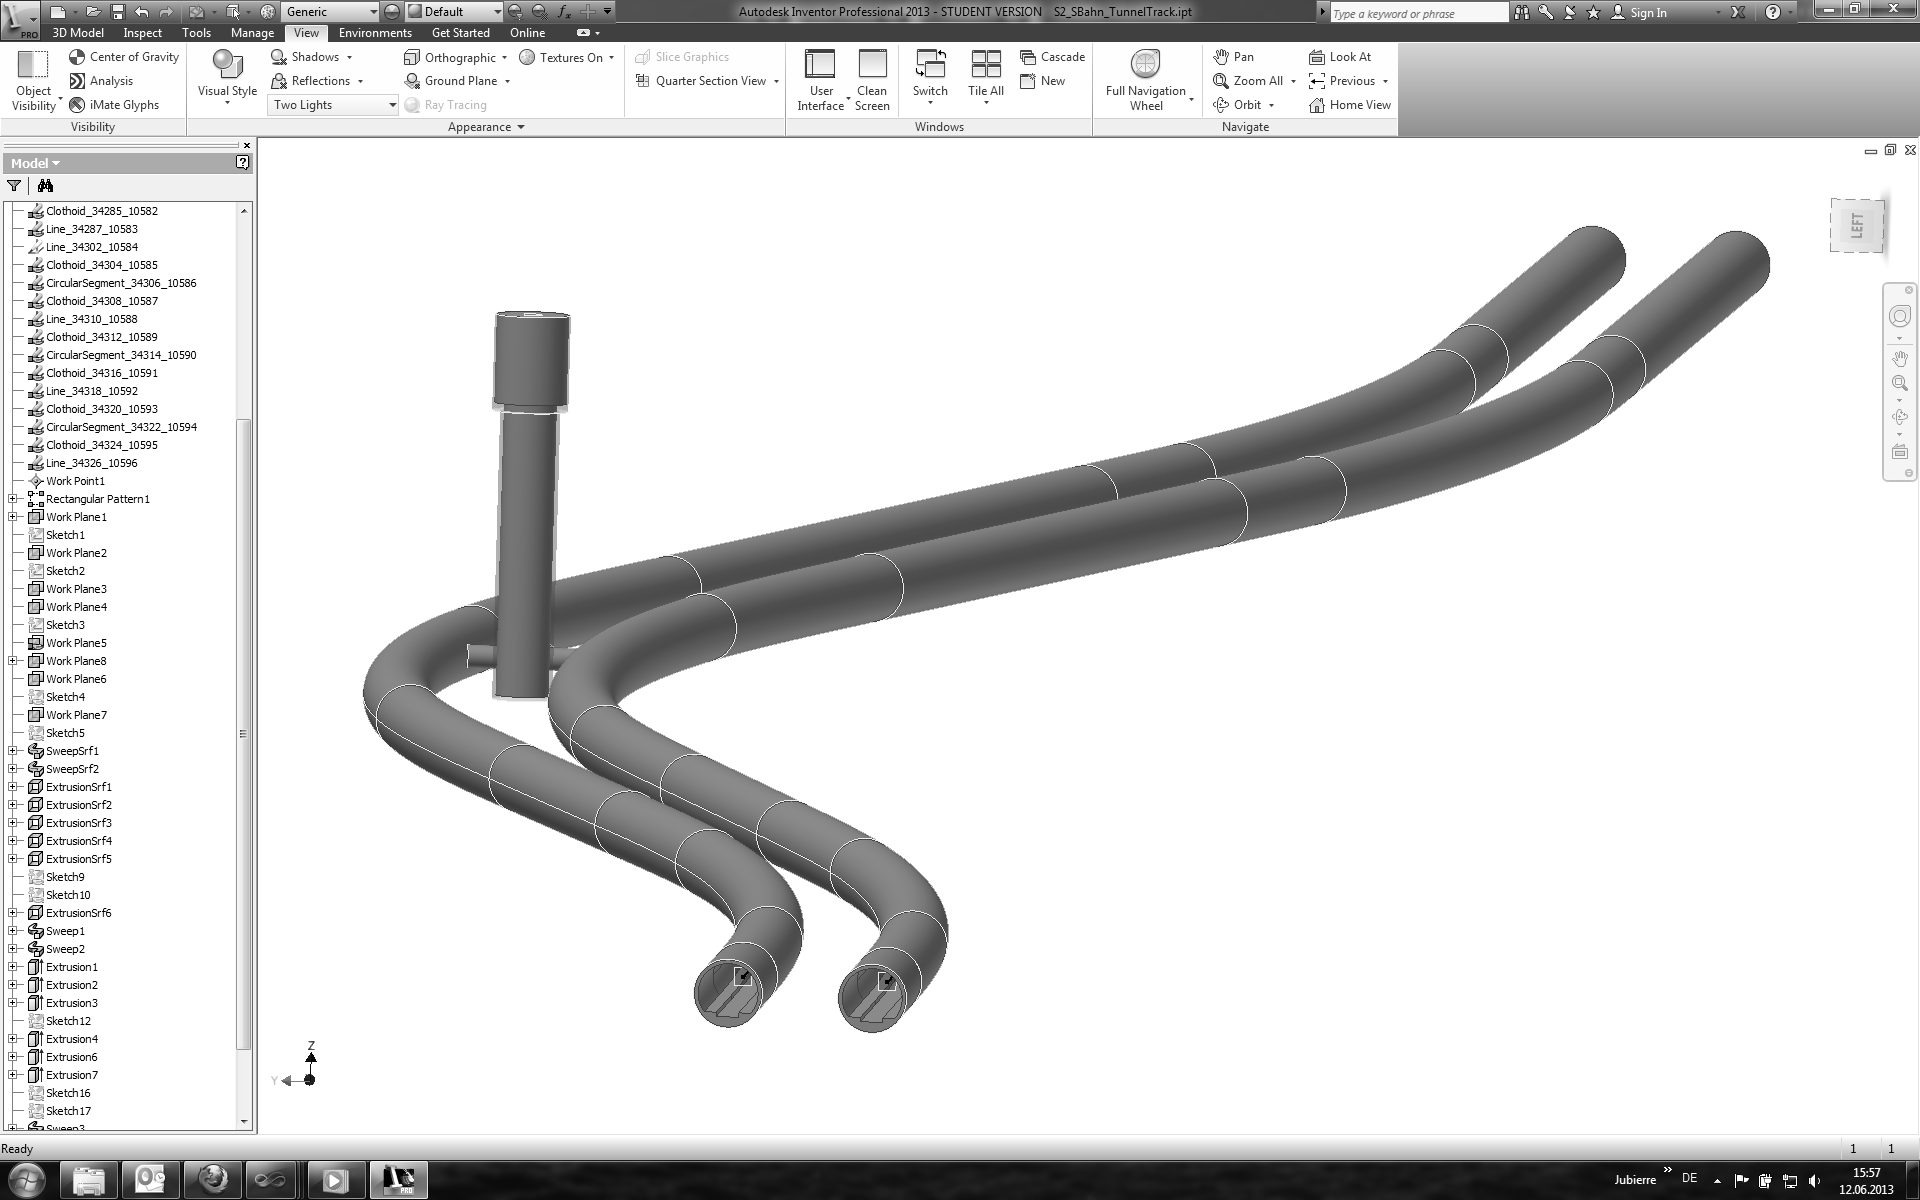
\includegraphics[width=140mm]{figure2.png}
%	\caption{Twin-Tunnel Model}
%	\label{figure:example2}
%	\end{center}
%\end{figure}
%
%\subsection{Formulas}
%
%Displayed equations or formulas are centered and set on a separate line (with an extra line or half-line space above and below). Displayed expressions should be numbered for reference. The numbers should be consecutive within each section or within the contribution, with numbers enclosed in parentheses and set on the right margin. 
%
%\subsection{Program Code}
%
%Program listings or program commands in the text are normally set in courier font point 9. However try to avoid “Copy-Paste” code, as they need a lot of space and usually are difficult to follow. Use in such a cases UML diagrams or pseudo-code.
%
%\subsection{Citations and References}
%
%The Harvard referencing style must be used, e.g. \citealp{Ashrae2005}. Another cite with parentheses \citep{Mawdesley2004}. The list of references is headed “References” and is not assigned a number in the decimal system of headings. The list should be set in small print and placed at the end of your contribution, in front of the appendix, if one exists. Please do not insert a page break before the list of references if the page is not completely filled
%
%\section{Conclusions / Future work}
%
%At the end of the paper be sure you summarize the work done and that you give some hints for a future extension of your topic. 
%